\documentclass[11pt,a4paper]{article}

% ============================================================
% PACKAGES
% ============================================================

\usepackage[margin=1in]{geometry}
\usepackage{lmodern}
\usepackage[T1]{fontenc}
\usepackage[utf8]{inputenc}
\usepackage{microtype}

\usepackage{amsmath}
\usepackage{amssymb}
\usepackage{graphicx} % Added for scaling large TikZ diagrams

\usepackage{booktabs}
\usepackage{longtable}
\usepackage{array}

\usepackage{xcolor}
\usepackage{hyperref}
\usepackage{enumitem}
\usepackage{listings}

\usepackage{tikz}
\usetikzlibrary{
arrows.meta,
positioning,
shapes.geometric,
shapes.misc,
fit,
backgrounds,
calc
}

\hypersetup{
colorlinks=true,
linkcolor=blue,
citecolor=blue,
urlcolor=blue,
pdftitle={OpenTelemetry, AI Observability, and Governance Audits},
pdfauthor={Mahua Banerjee}
}

% ============================================================
% LISTINGS
% ============================================================

\lstset{
basicstyle=\ttfamily\small,
breaklines=true,
frame=single,
columns=fullflexible
}

% ============================================================
% TITLE
% ============================================================

\title{
\textbf{OpenTelemetry, AI Observability, and Governance Audits}\\[0.5em]
\large A Student Reading Reference for LiteLLM, Langfuse, AgentOps, and LLM Governance
}

\author{Mahua Banerjee}

\date{\today}

\begin{document}

\maketitle

\begin{abstract}
Modern AI applications are not single model calls. A production AI request may travel through an agent workflow, invoke one or more tools, retrieve documents from a vector database, access memory, call an LLM through a provider abstraction layer, and finally produce an answer.

This creates a difficult operational question:

\begin{quote}
\textit{If an AI system produces an incorrect, unsafe, expensive, or policy-violating result, can we reconstruct what happened?}
\end{quote}

OpenTelemetry (OTel) provides a standardized way to describe and propagate telemetry across distributed systems. Langfuse builds AI-specific observability capabilities on top of OpenTelemetry concepts. LiteLLM can act as a model abstraction and routing layer through which model requests can be consistently observed and enriched with metadata.

This document explains the concepts of traces, spans, trace context, attributes, events, baggage, sessions, observations, metadata, and correlation identifiers. It then develops an architecture in which telemetry can become evidence for AI operations, debugging, evaluation, and governance audits.

The central argument is:

\[
\boxed{
\text{Observability}
\rightarrow
\text{Execution Visibility}
\rightarrow
\text{Evidence Collection}
\rightarrow
\text{Evaluation and Controls}
\rightarrow
\text{Auditability}
}
\]

Observability alone is not governance. However, without sufficiently structured execution evidence, meaningful technical governance and post-hoc auditing become substantially more difficult.
\end{abstract}

\tableofcontents
\newpage

% ============================================================
\section{Relationship to the Bootcamp}

This reading should be understood as connecting multiple days of the bootcamp rather than as an isolated OpenTelemetry topic.

\begin{table}[h]
\centering
\begin{tabular}{p{0.25\textwidth}p{0.65\textwidth}}
\toprule
\textbf{Bootcamp Area} & \textbf{Connection to this Reading} \\
\midrule
Day 12: Agent Memory &
Introduces the distinction between an execution trace and a longer-lived conversation or session. \\
\addlinespace
Days 15--21: RAG &
Retrieval, top-$k$ documents, context construction, and RAG evaluation can become observable operations. \\
\addlinespace
Day 22: LLMOps &
Introduces production concerns beyond simply generating an answer. \\
\addlinespace
Day 23: LiteLLM &
Provides provider abstraction and a potential common observation point for model calls. \\
\addlinespace
Day 24: Model Routing &
Telemetry can show which model was selected, why, how much it cost, and how it performed. \\
\addlinespace
Day 25: Langfuse &
Introduces traces, spans, token usage, cost, and AI-specific observability. \\
\addlinespace
Day 26: AgentOps &
Tool calls, memory, retrieval, execution paths, failures, and latency become observable. \\
\addlinespace
Day 27: Continuous Evaluation &
Telemetry can be correlated with evaluation scores, prompt versions, and regression evidence. \\
\addlinespace
Day 28: Final Capstone &
All of these concepts meet in one end-to-end production-style architecture. \\
\bottomrule
\end{tabular}
\end{table}

The bootcamp's final architecture is conceptually:

\[
\text{n8n}
+
\text{Qdrant}
+
\text{LiteLLM}
+
\text{Model Providers}
+
\text{Langfuse}
\]

The observability layer therefore should not be viewed as ``something added after the application works.'' It is part of the production architecture.

% ============================================================
\section{The Core Problem: AI Systems are Execution Graphs}

A simple chatbot may look like this:

\[
\text{User}
\rightarrow
\text{LLM}
\rightarrow
\text{Response}
\]

However, an agentic system may actually execute:

\[
\text{User}
\rightarrow
\text{Workflow}
\rightarrow
\text{Agent}
\rightarrow
\begin{cases}
\text{Memory Lookup}\\
\text{Retriever}\\
\text{Tool Call}\\
\text{LLM Call}\\
\text{Model Router}
\end{cases}
\rightarrow
\text{Response}
\]

A useful abstraction is to think of a request as producing an \textbf{execution graph}.

For a request $R$:

\[
R = \{o_1, o_2, o_3, \ldots, o_n\}
\]

where each $o_i$ is an operation.

For example:

\[
R =
\left\{
\begin{aligned}
&\text{Receive Query}, \text{Load Memory}, \text{Retrieve Documents}, \\
&\text{Build Prompt}, \text{LLM Generation}, \text{Tool Call}, \text{Final Response}
\end{aligned}
\right\}
\]

The central observability problem is therefore:

\begin{quote}
How can all of these operations be connected so that they can later be understood as one coherent execution?
\end{quote}

OpenTelemetry provides the fundamental answer through \textbf{traces}, \textbf{spans}, and \textbf{context propagation}.

% ============================================================
\section{What is OpenTelemetry?}

OpenTelemetry, commonly abbreviated as OTel, is an open observability framework and specification.

It provides a standardized approach for collecting and propagating telemetry such as:

\begin{itemize}
\item traces,
\item spans,
\item metrics,
\item logs,
\item context,
\item baggage,
\item resource information.
\end{itemize}

The important architectural idea is:

\[
\boxed{
\text{Instrumentation}
\rightarrow
\text{Standard Telemetry}
\rightarrow
\text{Export}
\rightarrow
\text{Observability Backend}
}
\]

For example:

\[
\text{Application}
\rightarrow
\text{OTel Instrumentation}
\rightarrow
\text{OTLP}
\rightarrow
\text{Langfuse / Collector / Other Backend}
\]

OTel is not itself primarily an AI governance product.

Instead, it provides a common language for representing what happened inside a distributed system.

For AI applications, this is increasingly important because a single user request may involve multiple services, models, tools, databases, and execution environments.

% ============================================================
\section{The Trace}

\subsection{Concept}

A \textbf{trace} represents the overall execution of a request or transaction.

For example:

\begin{quote}
``Answer the customer's question about the company's refund policy.''
\end{quote}

The complete lifecycle of handling this request can be represented as one trace.

\begin{center}
\resizebox{\linewidth}{!}{
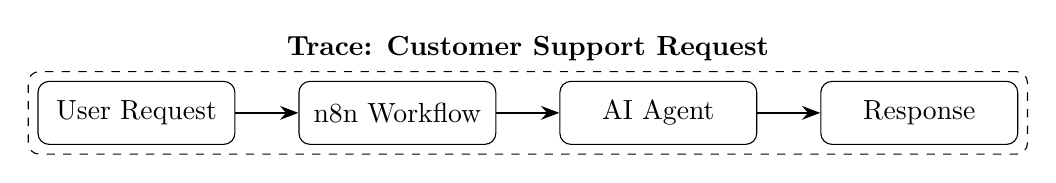
\begin{tikzpicture}[
node distance=0.8cm,
box/.style={
draw,
rounded corners,
minimum width=2.5cm,
minimum height=0.8cm,
align=center
},
arrow/.style={->,>=Stealth,thick}
]

\node[box] (user) {User Request};
\node[box,right=of user] (workflow) {n8n Workflow};
\node[box,right=of workflow] (agent) {AI Agent};
\node[box,right=of agent] (response) {Response};

\draw[arrow] (user) -- (workflow);
\draw[arrow] (workflow) -- (agent);
\draw[arrow] (agent) -- (response);

\node[draw,dashed,rounded corners,fit=(user)(workflow)(agent)(response),
label=above:{\textbf{Trace: Customer Support Request}}] {};

\end{tikzpicture}
}
\end{center}

The trace is therefore the answer to:

\begin{quote}
\textit{What happened during this particular end-to-end execution?}
\end{quote}

Each trace has an identifier:

\[
\texttt{trace\_id}
\]

All operations belonging to the same distributed execution can be correlated using this identifier.

% ============================================================
\section{The Span}

\subsection{Concept}

A \textbf{span} represents one unit of work within a trace.

Suppose an agent handles a customer request.

The trace might contain:

\begin{enumerate}
\item Receive Request
\item Retrieve Customer Memory
\item Retrieve Company Documents
\item Construct Prompt
\item Call LLM
\item Call CRM Tool
\item Generate Final Response
\end{enumerate}

Each of these can be represented as a span.

\begin{center}
\resizebox{\linewidth}{!}{
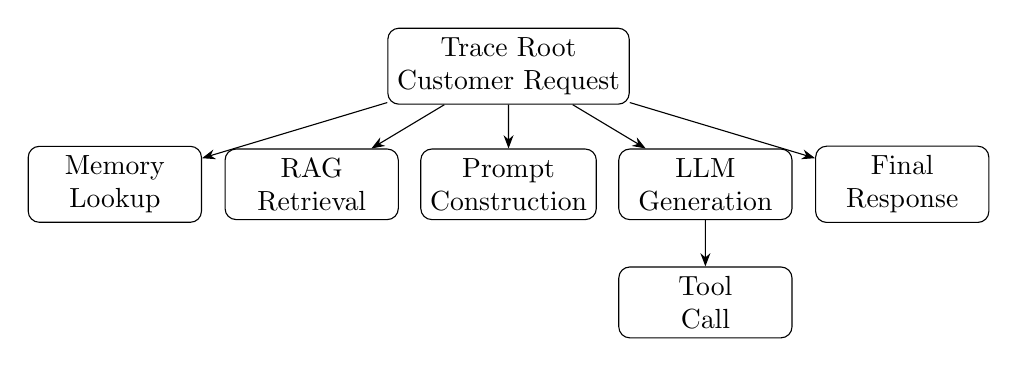
\begin{tikzpicture}[
level distance=1.5cm,
sibling distance=2.5cm,
edge from parent/.style={draw,->,>=Stealth},
every node/.style={
draw,
rounded corners,
align=center,
minimum width=2.2cm,
minimum height=0.8cm
}
]

\node {Trace Root\\Customer Request}
child {node {Memory\\Lookup}}
child {node {RAG\\Retrieval}}
child {node {Prompt\\Construction}}
child {node {LLM\\Generation}
child {node {Tool\\Call}}
}
child {node {Final\\Response}};

\end{tikzpicture}
}
\end{center}

Formally, a trace can be represented as:

\[
T = \{S_1, S_2, \ldots, S_n\}
\]

where each $S_i$ is a span.

A span generally contains information such as:

\[
S =
(
\text{name},
\text{span\_id},
\text{parent\_span\_id},
t_{start},
t_{end},
\text{attributes},
\text{events},
\text{status}
)
\]

The duration of a span is:

\[
\text{Latency}(S) = t_{end} - t_{start}
\]

This immediately allows operational questions such as:

\begin{itemize}
\item Which operation was slow?
\item Which model call failed?
\item How long did retrieval take?
\item Which tool caused the workflow to fail?
\end{itemize}

% ============================================================
\section{Parent--Child Relationships}

Spans are normally connected through parent--child relationships.

For example:

\[
S_{workflow}
\rightarrow
S_{agent}
\rightarrow
S_{retrieval}
\]

or:

\[
S_{agent}
\rightarrow
S_{generation}
\rightarrow
S_{tool}
\]

This produces a trace tree.

The trace tree answers questions that ordinary logs often struggle to answer:

\begin{quote}
``This LLM call took five seconds---but which user request caused it, which agent invoked it, and what happened before and after it?''
\end{quote}

The parent--child structure preserves execution context.

% ============================================================
\section{Trace Context and Context Propagation}

The trace must continue across process boundaries.

Consider:

\[
\text{n8n}
\rightarrow
\text{LiteLLM Proxy}
\rightarrow
\text{Model Provider}
\]

These may be separate processes or services.

Without context propagation, each system could produce isolated telemetry.

We might observe:

\[
T_1 = \text{n8n request}
\]

and separately:

\[
T_2 = \text{LiteLLM model request}
\]

and separately:

\[
T_3 = \text{provider response}
\]

But we would not necessarily know:

\[
T_1 \leftrightarrow T_2 \leftrightarrow T_3
\]

Context propagation attempts to preserve the relationship.

Conceptually:

\[
\boxed{
\text{Trace Context} = (
\text{trace\_id},
\text{current span identity},
\text{other propagation state}
)
}
\]

When service $A$ calls service $B$, relevant context can be injected into the outgoing request.

Service $B$ extracts the context and creates a child span.

Thus:

\[
S_A
\rightarrow
S_B
\]

even though:

\[
A \neq B
\]

This is one of the fundamental reasons distributed tracing is useful.

% ============================================================
\section{SpanContext}

A \textbf{SpanContext} contains the identifying information needed to propagate tracing relationships.

The important identifiers are:

\begin{itemize}
\item \texttt{trace\_id}
\item \texttt{span\_id}
\end{itemize}

Conceptually:

\[
\text{Trace} = \text{All spans sharing the same trace identifier}
\]

while:

\[
\text{Span} = \text{One identifiable operation within that trace}
\]

For example:

\begin{lstlisting}
trace_id = abc123

span_1 = Receive Request
span_2 = Retrieve Documents
span_3 = LLM Generation
span_4 = CRM Tool Call
\end{lstlisting}

All spans can belong to:

\begin{lstlisting}
trace_id = abc123
\end{lstlisting}

This is what enables an observability platform to reconstruct the execution tree.

% ============================================================
\section{Attributes: Adding Meaning to Telemetry}

A trace identifier tells us:

\begin{quote}
``These operations belong together.''
\end{quote}

But it does not tell us:

\begin{quote}
``What was the model?''
\end{quote}

or:

\begin{quote}
``Which prompt version was used?''
\end{quote}

or:

\begin{quote}
``Was this request from the production environment?''
\end{quote}

This is where \textbf{attributes} become important.

An attribute is generally a key--value pair.

For example:

\begin{lstlisting}
model = "gpt-4o"
environment = "production"
prompt_version = "v12"
tenant_id = "enterprise_42"
risk_level = "high"
\end{lstlisting}

Mathematically:

\[
A(S) = \{ (k_1,v_1), (k_2,v_2), \ldots, (k_n,v_n) \}
\]

where $A(S)$ is the attribute set associated with span $S$.

Attributes transform raw telemetry into structured evidence.

Compare:

\begin{quote}
LLM call failed.
\end{quote}

with:

\begin{lstlisting}
trace_id       = abc123
model          = gpt-4o
provider       = openai
environment    = production
prompt_version = v12
workflow       = customer-support
tenant         = enterprise_42
operation      = refund-analysis
error          = timeout
\end{lstlisting}

The second record is much more useful operationally and potentially more useful during an audit.

% ============================================================
\section{Events}

A span describes an operation with duration.

An \textbf{event} can represent something that happened at a particular point in time during that operation.

For example, inside an agent execution span:

\begin{lstlisting}
10:00:01  agent.started
10:00:02  retrieval.completed
10:00:03  tool.selected
10:00:04  tool.failed
10:00:05  fallback.triggered
\end{lstlisting}

Events can help answer:

\begin{itemize}
\item When did a failure occur?
\item When did the agent change strategy?
\item When was fallback activated?
\item When was a policy control triggered?
\end{itemize}

For governance purposes, events can potentially represent important control points:

\[
\text{Execution}
\rightarrow
\text{Policy Check Event}
\rightarrow
\text{Evaluation Event}
\rightarrow
\text{Fallback Event}
\]

However, whether a platform records these automatically depends on the application's instrumentation.

% ============================================================
\section{Baggage}

Baggage is contextual key--value information that can travel alongside distributed context.

Conceptually:

\[
B = \{ (k_1,v_1), (k_2,v_2), \ldots \}
\]

Suppose an incoming request contains:

\begin{lstlisting}
tenant_id = bank_42
application_id = loan-agent
environment = production
\end{lstlisting}

This contextual information may need to be available downstream.

For example:

\[
\text{n8n}
\rightarrow
\text{LiteLLM}
\rightarrow
\text{Tool Service}
\]

Baggage can conceptually help carry context across the chain.

However, an important distinction must be understood:

\[
\boxed{
\text{Baggage} \neq \text{Span Attributes}
}
\]

Baggage is propagated contextual information.

It must be explicitly used or copied into telemetry attributes if the implementation requires it to become queryable observation data.

Students should also understand the security implication:

\begin{quote}
Do not treat baggage as a secure transport for sensitive data.
\end{quote}

Sensitive information should be minimized, classified, and protected according to the application's security and privacy requirements.

% ============================================================
\section{Resources: What Produced the Telemetry?}

A \textbf{resource} describes the entity producing telemetry.

Examples:

\begin{itemize}
\item application,
\item service,
\item container,
\item virtual machine,
\item Kubernetes workload,
\item environment.
\end{itemize}

Conceptually:

\[
\text{Telemetry Record} = \text{Execution Data} + \text{Resource Context}
\]

For example:

\begin{lstlisting}
service.name = litellm-proxy
deployment.environment = production
host.name = ai-gateway-01
service.version = 1.8.2
\end{lstlisting}

This is important because governance questions often require distinguishing:

\[
\text{Development} \neq \text{Testing} \neq \text{Production}
\]

A trace from an experimental environment should not automatically be interpreted in the same way as production evidence.

% ============================================================
\section{Sessions: A Different Concept from Traces}

Students frequently confuse a \textbf{trace} with a \textbf{session}.

They are not the same.

\subsection{Trace}

A trace normally represents one end-to-end execution.

For example:

\[
\text{One User Request}
\rightarrow
\text{One Trace}
\]

\subsection{Session}

A session can represent a longer-running interaction.

For example:

\[
\text{Customer Conversation} = \{ T_1,T_2,T_3,T_4,T_5 \}
\]

where:

\[
T_i = \text{individual request trace}
\]

Consider:

\begin{center}
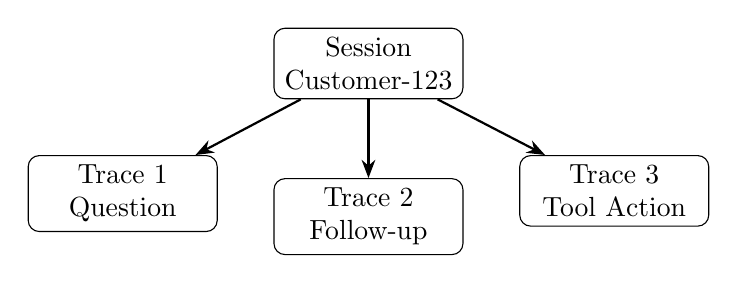
\begin{tikzpicture}[
node distance=1cm,
box/.style={
draw,
rounded corners,
minimum width=2.4cm,
minimum height=0.8cm,
align=center
},
arrow/.style={->,>=Stealth,thick}
]

\node[box] (session) {Session\\Customer-123};

\node[box,below left=of session] (t1) {Trace 1\\Question};
\node[box,below=of session] (t2) {Trace 2\\Follow-up};
\node[box,below right=of session] (t3) {Trace 3\\Tool Action};

\draw[arrow] (session) -- (t1);
\draw[arrow] (session) -- (t2);
\draw[arrow] (session) -- (t3);

\end{tikzpicture}
\end{center}

Therefore:

\[
\boxed{
\text{Session} = \text{Collection of related traces over time}
}
\]

This aligns conceptually with the bootcamp's Day 12 discussion of conversational state and session memory.

However, the following distinction is important:

\[
\text{Session ID} \neq \text{Memory Store}
\]

A session identifier helps correlate interactions.

Memory is actual state or information available to the agent.

% ============================================================
\section{AI-Specific Observability}

Traditional distributed tracing might contain operations such as:

\begin{itemize}
\item HTTP request,
\item database query,
\item cache lookup,
\item RPC call.
\end{itemize}

AI systems introduce additional operations:

\begin{itemize}
\item LLM inference,
\item embeddings,
\item vector retrieval,
\item context construction,
\item agent planning,
\item memory retrieval,
\item tool execution,
\item evaluation.
\end{itemize}

Conceptually, a GenAI trace can therefore be represented as:

\[
T = \{ S_{workflow}, S_{memory}, S_{retrieval}, S_{prompt}, S_{generation}, S_{tool}, S_{evaluation} \}
\]

Recent OpenTelemetry work includes evolving semantic conventions for GenAI operations.

The goal of semantic conventions is standardization.

Instead of every organization inventing:

\begin{lstlisting}
my_model_name
ai_model
llm_name
used_model
\end{lstlisting}

a common semantic vocabulary can improve interoperability.

% ============================================================
\section{Why Semantic Conventions Matter}

Suppose three systems record model information differently:

\begin{lstlisting}
System A:
model = gpt-4o

System B:
llm_model = gpt-4o

System C:
selected_model = gpt-4o
\end{lstlisting}

Aggregating this data is inconvenient.

Semantic conventions attempt to standardize meaning.

The general principle is:

\[
\boxed{
\text{Standardized Names}
\rightarrow
\text{Better Correlation}
\rightarrow
\text{Better Aggregation}
\rightarrow
\text{Better Interoperability}
}
\]

This becomes particularly valuable in a multi-vendor architecture.

For example:

\[
\text{n8n}
\rightarrow
\text{LiteLLM}
\rightarrow
\text{OpenAI}
\]

or:

\[
\text{n8n}
\rightarrow
\text{LiteLLM}
\rightarrow
\text{Ollama}
\]

A consistent telemetry vocabulary can make cross-provider analysis easier.

% ============================================================
\section{Langfuse and OpenTelemetry}

Langfuse provides AI-specific observability capabilities while building its SDK architecture around OpenTelemetry concepts.

Conceptually:

\[
\text{OTel Trace} \approx \text{Langfuse Trace}
\]

and:

\[
\text{OTel Span} \approx \text{Langfuse Observation}
\]

Langfuse further specializes observations.

For example:

\[
\text{Observation} \in \{ \text{Span}, \text{Generation}, \text{Event}, \text{Tool}, \text{Retrieval} \}
\]

An LLM generation is more specialized than a generic span because it may contain AI-specific information:

\[
G = ( \text{model}, \text{parameters}, \text{token usage}, \text{cost}, \text{latency}, \text{input}, \text{output} )
\]

This is one reason AI observability platforms provide more useful abstractions for LLM applications than generic APM systems alone.

% ============================================================
\section{Trace-Level Correlation in Langfuse}

A Langfuse trace can contain shared information such as:

\begin{itemize}
\item user identifier,
\item session identifier,
\item metadata,
\item tags,
\item version,
\item environment.
\end{itemize}

Conceptually:

\[
T = ( \text{trace\_id}, \text{user\_id}, \text{session\_id}, \text{metadata}, \text{tags}, \text{observations} )
\]

This enables questions such as:

\begin{quote}
Show all failed traces associated with:
\end{quote}

\begin{lstlisting}
environment = production
application = customer-support
prompt_version = v12
model = gpt-4o
\end{lstlisting}

Or:

\begin{quote}
Calculate the average cost per session for a particular workflow.
\end{quote}

This is where metadata design becomes strategically important.

% ============================================================
\section{The LiteLLM Layer}

LiteLLM provides a model abstraction layer.

Conceptually:

\[
\text{Application}
\rightarrow
\text{LiteLLM}
\rightarrow
\begin{cases}
\text{OpenAI}\\
\text{Anthropic}\\
\text{Ollama}\\
\text{Other Providers}
\end{cases}
\]

The application can interact with a common interface while LiteLLM manages provider-specific behavior.

For the bootcamp architecture:

\[
\text{n8n Agent}
\rightarrow
\text{LiteLLM Proxy}
\rightarrow
\text{Selected Model}
\]

This makes LiteLLM strategically interesting for observability because it can become a common point through which model requests flow.

Instead of instrumenting every possible provider independently, the model gateway can become an important observation boundary.

% ============================================================
\section{LiteLLM as an Observability Boundary}

Consider the following architecture:

\begin{center}
\resizebox{\linewidth}{!}{
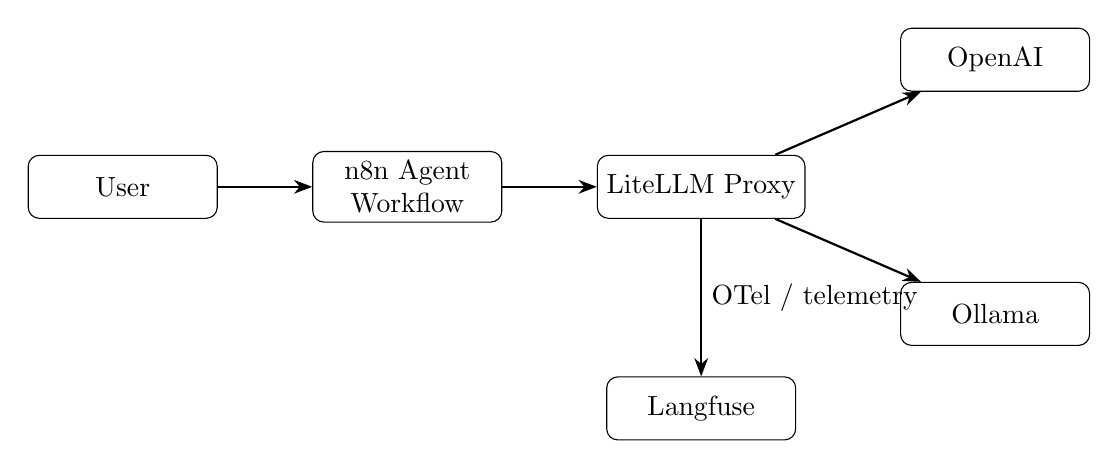
\begin{tikzpicture}[
node distance=1.2cm,
box/.style={
draw,
rounded corners,
minimum width=2.4cm,
minimum height=0.8cm,
align=center
},
arrow/.style={->,>=Stealth,thick}
]

\node[box] (user) {User};
\node[box,right=of user] (n8n) {n8n Agent\\Workflow};
\node[box,right=of n8n] (litellm) {LiteLLM Proxy};

\node[box,above right=0.8cm and 1.2cm of litellm] (openai) {OpenAI};
\node[box,below right=0.8cm and 1.2cm of litellm] (ollama) {Ollama};

\node[box,below=2cm of litellm] (langfuse) {Langfuse};

\draw[arrow] (user) -- (n8n);
\draw[arrow] (n8n) -- (litellm);
\draw[arrow] (litellm) -- (openai);
\draw[arrow] (litellm) -- (ollama);

\draw[arrow] (litellm) -- node[right]{OTel / telemetry} (langfuse);

\end{tikzpicture}
}
\end{center}

The important design idea is:

\[
\boxed{
\text{Model Gateway} = \text{Potential Central Observation Point}
}
\]

LiteLLM can potentially expose information such as:

\begin{itemize}
\item selected model,
\item provider,
\item request timing,
\item token usage,
\item cost,
\item errors,
\item metadata supplied by the calling application.
\end{itemize}

This does not automatically mean LiteLLM observes the entire n8n workflow.

For full end-to-end visibility, instrumentation and correlation must extend across the relevant components.

% ============================================================
\section{Metadata: The Foundation of Correlation}

The most important practical lesson for governance-oriented observability is:

\[
\boxed{
\text{Telemetry without meaningful metadata has limited audit value.}
}
\]

Suppose we only record:

\begin{lstlisting}
model = gpt-4o
latency = 2.4 seconds
cost = $0.03
\end{lstlisting}

We know something about the model call.

But we may not know:

\begin{itemize}
\item Which application generated it?
\item Which workflow generated it?
\item Which prompt version was used?
\item Which model routing policy selected the model?
\item Was it development or production?
\item Which evaluation suite was associated with the deployment?
\item Which governance policy applied?
\end{itemize}

A stronger metadata model might be:

\begin{lstlisting}
application.name       = customer-support-agent
application.version    = 2.4.1

environment            = production

workflow.id            = refund-workflow
workflow.version       = 14

agent.id               = support-agent
agent.version          = 3.2

prompt.name            = refund-analysis
prompt.version         = v12

model.alias            = complex-task
model.selected         = gpt-4o
provider               = openai

evaluation.dataset     = refund-regression-set
evaluation.version     = 5

governance.policy      = customer-data-policy-v3
risk.classification    = medium

session_id             = session_123
tenant_id              = tenant_456
\end{lstlisting}

The objective is not to record everything.

The objective is to record enough structured information to answer important questions later.

% ============================================================
\section{Metadata Dimensions for AI Governance}

A useful metadata taxonomy is:

\subsection{1. Identity}

What system produced this event?

\begin{lstlisting}
application.id
workflow.id
agent.id
service.name
\end{lstlisting}

\subsection{2. Version}

Which version was running?

\begin{lstlisting}
application.version
workflow.version
prompt.version
agent.version
\end{lstlisting}

\subsection{3. Model}

Which AI system was used?

\begin{lstlisting}
model.alias
model.name
provider
routing.policy
\end{lstlisting}

\subsection{4. Context}

What kind of execution was this?

\begin{lstlisting}
environment
tenant_id
session_id
request_type
\end{lstlisting}

\subsection{5. Governance}

Which controls or policies were relevant?

\begin{lstlisting}
risk.classification
policy.id
policy.version
approval.status
data.classification
\end{lstlisting}

\subsection{6. Evaluation}

What quality evidence is associated with this execution?

\begin{lstlisting}
evaluation.dataset
evaluation.version
faithfulness.score
context_precision.score
pass_fail
\end{lstlisting}

This taxonomy connects directly to the bootcamp's progression from evaluation to RAGOps, AgentOps, PromptOps, ModelOps, and continuous evaluation.

% ============================================================
\section{A Complete Correlation Model}

A robust AI system may need several identifiers.

For example:

\[
\text{Session ID} \rightarrow \text{Conversation}
\]
\[
\text{Trace ID} \rightarrow \text{Single Execution}
\]
\[
\text{Span ID} \rightarrow \text{Individual Operation}
\]
\[
\text{Prompt Version} \rightarrow \text{Prompt Artifact}
\]
\[
\text{Model Version/Alias} \rightarrow \text{Model Selection}
\]
\[
\text{Evaluation Run ID} \rightarrow \text{Quality Evidence}
\]

These can be represented as a correlation graph:

\begin{center}
\resizebox{\linewidth}{!}{
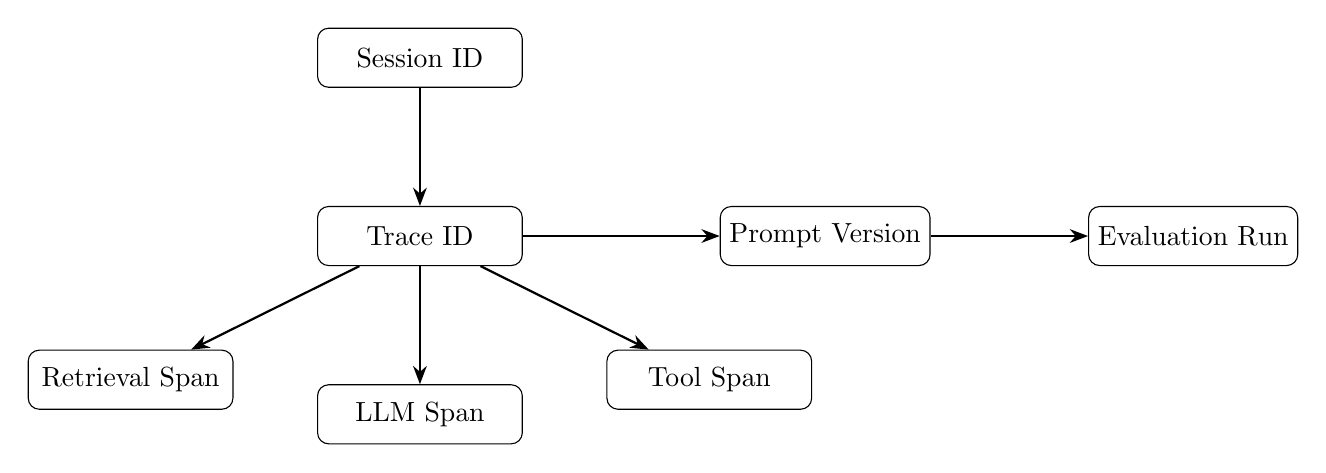
\begin{tikzpicture}[
node distance=1.5cm,
box/.style={
draw,
rounded corners,
minimum width=2.6cm,
minimum height=0.75cm,
align=center
},
arrow/.style={->,>=Stealth,thick}
]

\node[box] (session) {Session ID};
\node[box,below=of session] (trace) {Trace ID};
\node[box,below left=of trace] (span1) {Retrieval Span};
\node[box,below=of trace] (span2) {LLM Span};
\node[box,below right=of trace] (span3) {Tool Span};

\node[box,right=2.5cm of trace] (prompt) {Prompt Version};
\node[box,right=2.0cm of prompt] (eval) {Evaluation Run};

\draw[arrow] (session) -- (trace);
\draw[arrow] (trace) -- (span1);
\draw[arrow] (trace) -- (span2);
\draw[arrow] (trace) -- (span3);

\draw[arrow] (trace) -- (prompt);
\draw[arrow] (prompt) -- (eval);

\end{tikzpicture}
}
\end{center}

This supports a governance-oriented question such as:

\begin{quote}
``Show me all production executions of Agent A using Prompt Version 12 where the faithfulness score dropped below the approved threshold.''
\end{quote}

Without correlation identifiers and metadata, answering this may require manual forensic investigation.

% ============================================================
\section{Filtering}

Filtering means selecting telemetry records based on attributes.

For example:

\[
\text{environment} = \text{production}
\]

or:

\[
\text{model} = \text{gpt-4o}
\]

or:

\[
\text{prompt.version} = \text{v12}
\]

A conceptual query:

\begin{lstlisting}
environment = "production"
AND
workflow = "customer-support"
AND
prompt_version = "v12"
AND
error = true
\end{lstlisting}

Filtering is useful for:

\begin{itemize}
\item incident investigation,
\item regression analysis,
\item cost analysis,
\item governance review,
\item deployment comparison.
\end{itemize}

% ============================================================
\section{Aggregation}

Aggregation means computing information across multiple executions.

Suppose $N$ requests use model $M$.

Average latency:

\[
\bar{L}_M = \frac{1}{N} \sum_{i=1}^{N} L_i
\]

Total cost:

\[
C_M = \sum_{i=1}^{N} c_i
\]

Failure rate:

\[
F_M = \frac{\text{Number of Failed Executions}}{\text{Total Executions}}
\]

Average faithfulness:

\[
\bar{F} = \frac{1}{N} \sum_{i=1}^{N} F_i
\]

Now consider grouping by prompt version:

\[
\bar{F}_{v11} \quad vs \quad \bar{F}_{v12}
\]

This begins to connect observability with continuous evaluation.

% ============================================================
\section{From Traces to AI Governance Evidence}

An AI audit may ask questions such as:

\begin{itemize}
\item What system made this decision?
\item Which model was used?
\item Which prompt version was active?
\item What external information was retrieved?
\item Were tools invoked?
\item What controls were triggered?
\item Was the system evaluated before deployment?
\item Were quality thresholds met?
\item Did the production system deviate from expected behavior?
\end{itemize}

A trace can potentially provide part of the answer.

Consider:

\[
\text{Audit Question}
\rightarrow
\text{Required Evidence}
\rightarrow
\text{Telemetry Correlation}
\]

For example:

\begin{table}[h]
\centering
\begin{tabular}{p{0.36\textwidth}p{0.50\textwidth}}
\toprule
\textbf{Audit Question} & \textbf{Potential Technical Evidence} \\
\midrule
Which workflow executed? &
Workflow ID and version metadata. \\
\addlinespace
Which model responded? &
Model and provider metadata. \\
\addlinespace
What happened during execution? &
Trace and span hierarchy. \\
\addlinespace
Was retrieval involved? &
Retrieval span and associated metadata. \\
\addlinespace
Were external tools called? &
Tool execution observations. \\
\addlinespace
How expensive was execution? &
Token usage and cost information. \\
\addlinespace
Was the system evaluated? &
Evaluation run and score metadata. \\
\addlinespace
Did policy controls activate? &
Policy-related events or attributes. \\
\bottomrule
\end{tabular}
\end{table}

The critical word is \textbf{potential}.

Telemetry is not automatically sufficient evidence for every audit requirement.

Governance evidence may also require:

\begin{itemize}
\item access control records,
\item approval workflows,
\item model inventory,
\item risk assessments,
\item evaluation reports,
\item policy documents,
\item change management records,
\item retention controls,
\item data governance records.
\end{itemize}

% ============================================================
\section{Observability is Not Governance}

This distinction is essential.

\subsection{Observability asks}

\begin{quote}
What happened?
\end{quote}

\subsection{Governance asks}

\begin{quote}
Should this system exist, who is responsible for it, what controls apply, was it appropriately evaluated, and can compliance or accountability be demonstrated?
\end{quote}

Therefore:

\[
\boxed{
\text{Telemetry} \neq \text{Governance}
}
\]

A better model is:

\[
\boxed{
\text{Governance Evidence} = f(
\text{Telemetry}, \text{Policies}, \text{Evaluations}, \text{Approvals}, \text{Risk Controls}, \text{Provenance}
)
}
\]

Telemetry becomes one important evidence stream.

% ============================================================
\section{A Governance-Oriented Architecture}

Consider the following architecture.

\begin{center}
\resizebox{\linewidth}{!}{
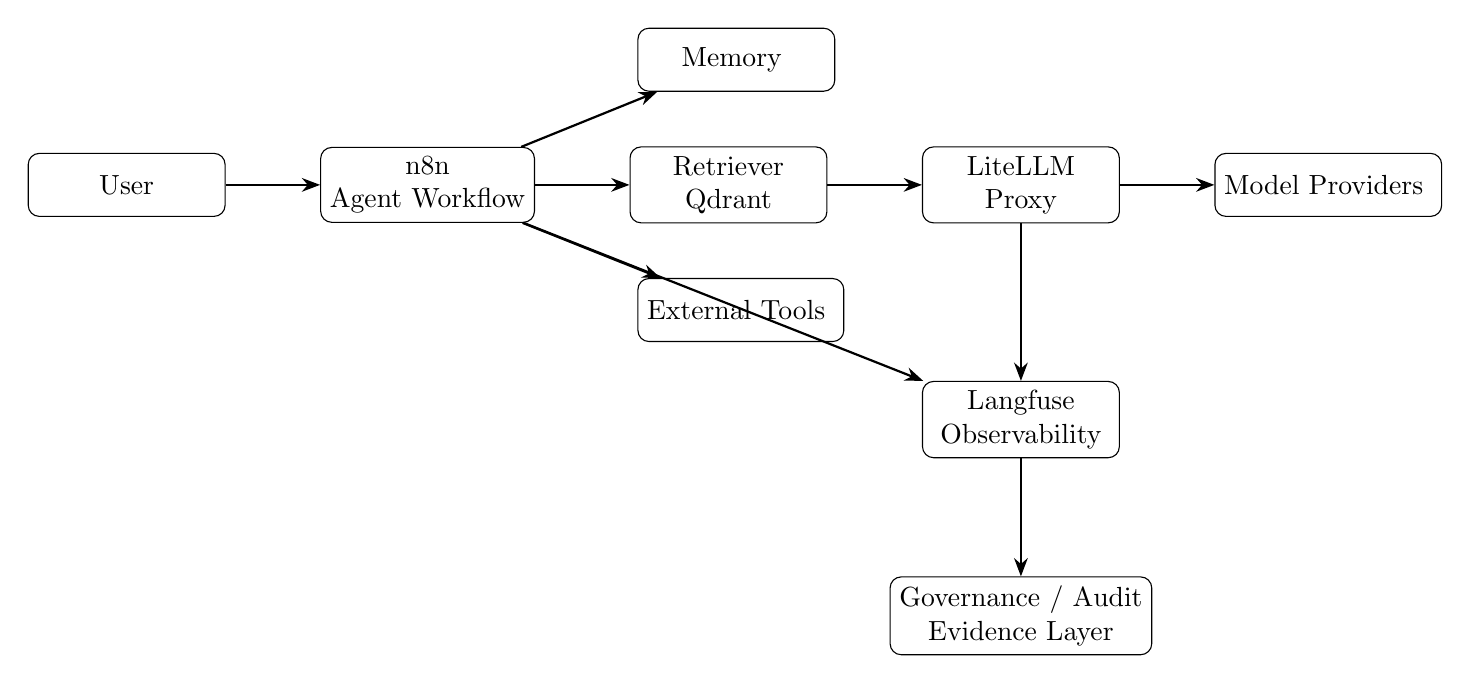
\begin{tikzpicture}[
node distance=1.2cm,
box/.style={
draw,
rounded corners,
minimum width=2.5cm,
minimum height=0.8cm,
align=center
},
arrow/.style={->,>=Stealth,thick}
]

\node[box] (user) {User};

\node[box,right=of user] (n8n) {
n8n\\
Agent Workflow
};

\node[box,above right=0.7cm and 1.3cm of n8n] (memory) {
Memory
};

\node[box,right=of n8n] (rag) {
Retriever\\
Qdrant
};

\node[box,below right=0.7cm and 1.3cm of n8n] (tools) {
External Tools
};

\node[box,right=of rag] (litellm) {
LiteLLM\\
Proxy
};

\node[box,right=of litellm] (models) {
Model Providers
};

\node[box,below=2cm of litellm] (langfuse) {
Langfuse\\
Observability
};

\node[box,below=1.5cm of langfuse] (governance) {
Governance / Audit\\
Evidence Layer
};

\draw[arrow] (user) -- (n8n);
\draw[arrow] (n8n) -- (memory);
\draw[arrow] (n8n) -- (rag);
\draw[arrow] (n8n) -- (tools);
\draw[arrow] (rag) -- (litellm);
\draw[arrow] (litellm) -- (models);

\draw[arrow] (n8n) -- (langfuse);
\draw[arrow] (litellm) -- (langfuse);
\draw[arrow] (langfuse) -- (governance);

\end{tikzpicture}
}
\end{center}

The observability system receives structured execution information.

The governance layer may then consume:

\[
\begin{aligned}
&\text{Trace Evidence}\\
+&\text{Evaluation Evidence}\\
+&\text{Version Metadata}\\
+&\text{Policy Metadata}\\
+&\text{Deployment Metadata}
\end{aligned}
\]

to create a stronger audit trail.

% ============================================================
\section{Example: Investigating a Bad AI Response}

Suppose a customer receives an incorrect refund policy answer.

The trace might show:

\[
T_{123}
\]

with:

\[
S_1 = \text{User Request}
\]
\[
S_2 = \text{Memory Retrieval}
\]
\[
S_3 = \text{RAG Retrieval}
\]
\[
S_4 = \text{Prompt Construction}
\]
\[
S_5 = \text{LLM Generation}
\]

An investigator could potentially inspect:

\begin{enumerate}
\item Which documents were retrieved?
\item Was the correct document missing?
\item What prompt version was used?
\item Which model generated the answer?
\item Was a fallback model activated?
\item What evaluation score was associated with the release?
\end{enumerate}

The failure could be classified as:

\[
\text{Failure} \in \{ \text{Retrieval Failure}, \text{Prompt Failure}, \text{Model Failure}, \text{Tool Failure}, \text{Memory Failure}, \text{Workflow Failure} \}
\]

This is the connection between observability and systematic AgentOps debugging.

% ============================================================
\section{Example: RAG Audit Trail}

For the bootcamp's enterprise knowledge assistant:

\[
\text{Question} \rightarrow \text{Retriever} \rightarrow \text{Top-}k\text{ Documents} \rightarrow \text{LLM} \rightarrow \text{Answer}
\]

An observable execution might contain:

\begin{lstlisting}
Trace:
user_question

Span:
embedding_query

Span:
vector_search
top_k = 3

Span:
context_construction
retrieved_documents = [...]

Span:
llm_generation
model = ...
prompt_version = ...

Span:
evaluation
faithfulness = ...
context_precision = ...
\end{lstlisting}

This can support:

\[
\text{Answer} \leftarrow \text{Model} \leftarrow \text{Prompt} \leftarrow \text{Retrieved Context} \leftarrow \text{Knowledge Source}
\]

This begins to resemble an execution provenance chain.

% ============================================================
\section{Example: Model Routing Audit}

Suppose the routing logic is:

\[
\text{Simple Task} \rightarrow \text{Llama}
\]
\[
\text{Complex Task} \rightarrow \text{GPT-4o}
\]

The trace should ideally make the routing decision observable.

For example:

\begin{lstlisting}
routing.policy = complexity-router-v3
task.classification = complex
selected.model = gpt-4o
fallback.used = false
\end{lstlisting}

An audit or engineering investigation could ask:

\begin{quote}
Did the system actually follow its intended routing policy?
\end{quote}

This is different from merely recording:

\begin{lstlisting}
model = gpt-4o
\end{lstlisting}

The routing decision itself is operationally relevant.

% ============================================================
\section{Example: PromptOps and Traceability}

Day 27 introduces:

\begin{itemize}
\item prompt versioning,
\item prompt testing,
\item rollback.
\end{itemize}

A production trace should ideally be correlatable with a prompt artifact.

For example:

\[
\text{Production Trace} \rightarrow \text{Prompt Name} + \text{Prompt Version}
\]

Suppose:

\[
P_{11} \rightarrow \text{Faithfulness}=0.92
\]

while:

\[
P_{12} \rightarrow \text{Faithfulness}=0.76
\]

A regression becomes easier to detect if executions can be grouped by prompt version.

This leads to:

\[
\boxed{
\text{PromptOps} + \text{Observability} = \text{Operational Prompt Traceability}
}
\]

% ============================================================
\section{Connecting Evaluation to Observability}

The bootcamp introduces RAGAS-style evaluation concepts such as:

\begin{itemize}
\item faithfulness,
\item context precision,
\item answer relevance,
\item context recall.
\end{itemize}

These evaluation results should not necessarily remain isolated CSV values.

Conceptually:

\[
\text{Evaluation Result} \leftrightarrow \text{Prompt Version} \leftrightarrow \text{Model} \leftrightarrow \text{Dataset} \leftrightarrow \text{Deployment}
\]

A useful evaluation record could therefore include:

\begin{lstlisting}
evaluation.run_id
evaluation.dataset_version
prompt.version
model
faithfulness
context_precision
answer_relevance
pass_fail
\end{lstlisting}

This supports:

\[
\text{CI/CD} \rightarrow \text{Evaluation} \rightarrow \text{Threshold} \rightarrow \text{Deployment Decision}
\]

Later production telemetry can then be compared against pre-deployment evidence.

% ============================================================
\section{Continuous Evaluation and Governance}

A one-time evaluation answers:

\begin{quote}
``Did the system perform acceptably during this test?''
\end{quote}

Continuous evaluation attempts to answer:

\begin{quote}
``Is the system continuing to perform acceptably as prompts, models, data, and workflows change?''
\end{quote}

A governance-oriented lifecycle is:

\[
\text{Change} \rightarrow \text{Evaluation} \rightarrow \text{Pass/Fail} \rightarrow \text{Deploy} \rightarrow \text{Observe} \rightarrow \text{Detect Drift or Regression}
\]

This is significantly stronger than:

\[
\text{Build} \rightarrow \text{Deploy} \rightarrow \text{Hope}
\]

% ============================================================
\section{A Possible AI Audit Evidence Model}

A useful conceptual model is:

\[
E = \{ I, V, X, Q, C \}
\]

where:

\[
I = \text{Identity Evidence}
\]
\[
V = \text{Version Evidence}
\]
\[
X = \text{Execution Evidence}
\]
\[
Q = \text{Quality Evidence}
\]
\[
C = \text{Control Evidence}
\]

Therefore:

\[
\boxed{
\text{AI Audit Evidence} = I+V+X+Q+C
}
\]

Examples:

\subsection{Identity Evidence}

\begin{itemize}
\item Application ID
\item Agent ID
\item Workflow ID
\end{itemize}

\subsection{Version Evidence}

\begin{itemize}
\item Prompt version
\item Workflow version
\item Model alias
\item Application release
\end{itemize}

\subsection{Execution Evidence}

\begin{itemize}
\item Trace ID
\item Span hierarchy
\item Tool calls
\item Retrieval operations
\end{itemize}

\subsection{Quality Evidence}

\begin{itemize}
\item Evaluation dataset
\item Metric scores
\item Pass/fail thresholds
\end{itemize}

\subsection{Control Evidence}

\begin{itemize}
\item Policy checks
\item Guardrail events
\item Approval status
\item Risk classification
\end{itemize}

% ============================================================
\section{Important Limitations}

Students should avoid making the following incorrect claims.

\subsection{Incorrect Claim 1}

\begin{quote}
``If we have traces, we are compliant.''
\end{quote}

False.

Traces may provide useful evidence, but compliance depends on the applicable legal, regulatory, organizational, and technical requirements.

\subsection{Incorrect Claim 2}

\begin{quote}
``OTel automatically captures every part of my AI system.''
\end{quote}

False.

Instrumentation and integration determine what is observed.

Uninstrumented components can remain invisible.

\subsection{Incorrect Claim 3}

\begin{quote}
``A trace proves why the model made a decision.''
\end{quote}

Usually too strong.

A trace can show execution steps, inputs, outputs, tools, and context, but this is not equivalent to a complete explanation of internal model reasoning.

\subsection{Incorrect Claim 4}

\begin{quote}
``More telemetry is always better.''
\end{quote}

False.

Telemetry can create:

\begin{itemize}
\item privacy risks,
\item sensitive data exposure,
\item storage costs,
\item security risks,
\item excessive operational noise.
\end{itemize}

The goal is:

\[
\boxed{
\text{Sufficient, Structured, Protected Evidence}
}
\]

not unlimited data collection.

% ============================================================
\section{Privacy and Sensitive Data}

AI telemetry can contain:

\begin{itemize}
\item user prompts,
\item model outputs,
\item retrieved documents,
\item tool parameters,
\item identifiers.
\end{itemize}

Therefore:

\[
\text{Observability Data} \subseteq \text{Potentially Sensitive Data}
\]

Possible design controls include:

\begin{itemize}
\item data minimization,
\item PII masking,
\item selective content capture,
\item hashing or pseudonymization,
\item access controls,
\item retention policies,
\item environment separation.
\end{itemize}

This creates an important governance tension:

\[
\text{More Detail} \rightarrow \text{Better Debugging}
\]

but also potentially:

\[
\text{More Detail} \rightarrow \text{Higher Privacy Exposure}
\]

The engineering problem is therefore an optimization problem rather than a simple ``capture everything'' decision.

% ============================================================
\section{Recommended Metadata Contract}

For a production AI platform, define a metadata contract.

For example:

\begin{lstlisting}
REQUIRED:

application.id
environment
workflow.id
workflow.version
trace_id

RECOMMENDED:

agent.id
agent.version
prompt.name
prompt.version
model.alias
model.name
provider

GOVERNANCE:

risk.classification
policy.id
policy.version
data.classification

EVALUATION:

evaluation.dataset
evaluation.version
evaluation.run_id
\end{lstlisting}

This should ideally become a documented contract rather than arbitrary metadata added by individual developers.

% ============================================================
\section{The Complete Bootcamp Ecosystem}

The end-to-end ecosystem can be understood as:

\begin{center}
\resizebox{\linewidth}{!}{
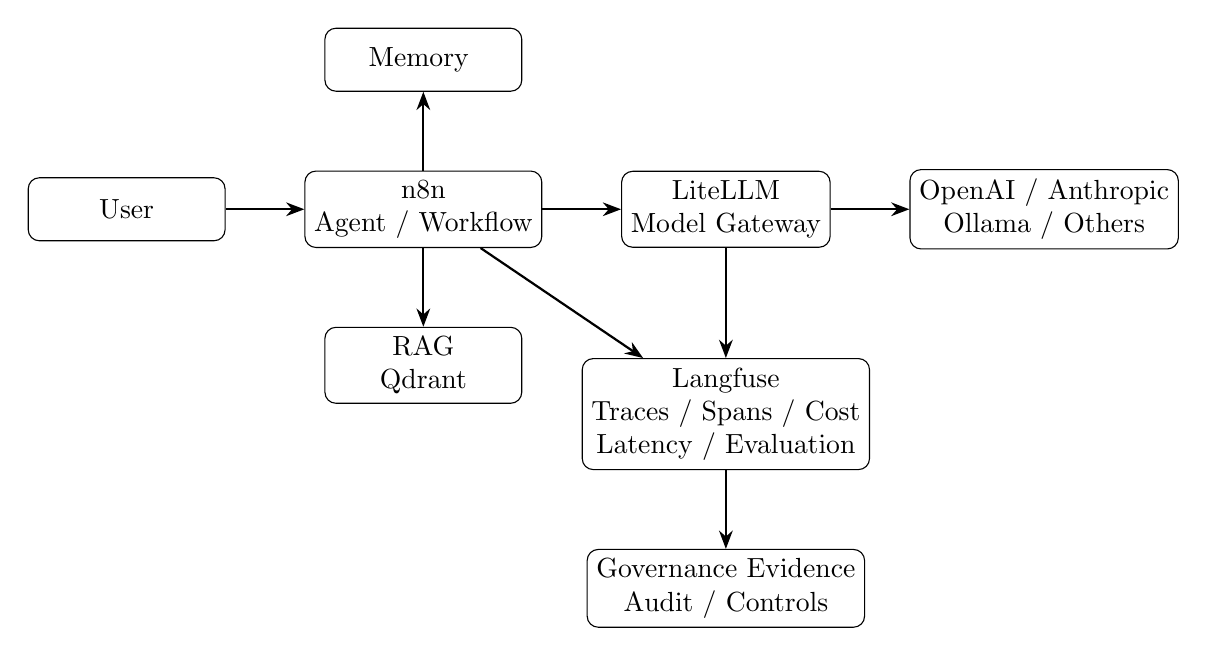
\begin{tikzpicture}[
node distance=1cm,
box/.style={
draw,
rounded corners,
minimum width=2.5cm,
minimum height=0.8cm,
align=center
},
arrow/.style={->,>=Stealth,thick}
]

\node[box] (user) {User};

\node[box,right=of user] (n8n) {
n8n\\
Agent / Workflow
};

\node[box,above=of n8n] (memory) {
Memory
};

\node[box,below=of n8n] (rag) {
RAG\\
Qdrant
};

\node[box,right=of n8n] (litellm) {
LiteLLM\\
Model Gateway
};

\node[box,right=of litellm] (models) {
OpenAI / Anthropic\\
Ollama / Others
};

\node[box,below=1.4cm of litellm] (langfuse) {
Langfuse\\
Traces / Spans / Cost\\
Latency / Evaluation
};

\node[box,below=of langfuse] (governance) {
Governance Evidence\\
Audit / Controls
};

\draw[arrow] (user) -- (n8n);
\draw[arrow] (n8n) -- (memory);
\draw[arrow] (n8n) -- (rag);
\draw[arrow] (n8n) -- (litellm);
\draw[arrow] (litellm) -- (models);

\draw[arrow] (n8n) -- (langfuse);
\draw[arrow] (litellm) -- (langfuse);

\draw[arrow] (langfuse) -- (governance);

\end{tikzpicture}
}
\end{center}

The conceptual flow is:

\[
\boxed{
\text{Agentic Execution}
\rightarrow
\text{Telemetry}
\rightarrow
\text{Observability}
\rightarrow
\text{Evaluation}
\rightarrow
\text{Governance Evidence}
}
\]

% ============================================================
\section{Key Takeaways}

Students should remember the following hierarchy.

\subsection*{Trace}

The complete lifecycle of one distributed execution.

\[
\text{One Request} \approx \text{One Trace}
\]

\subsection*{Span}

One operation inside that execution.

\[
\text{Trace} = \sum \text{Spans}
\]

conceptually speaking.

\subsection*{Context Propagation}

The mechanism that helps preserve execution relationships across components.

\[
\text{Service A} \rightarrow \text{Service B} \rightarrow \text{Service C}
\]

while maintaining the execution relationship.

\subsection*{Attributes}

Structured metadata describing operations.

\[
\text{Span} + \text{Attributes} = \text{Meaningful Operational Record}
\]

\subsection*{Session}

A longer-lived grouping of multiple related traces.

\[
\text{Session} = \{T_1,T_2,\ldots,T_n\}
\]

\subsection*{LiteLLM}

A model abstraction and gateway layer that can act as an important common observation point for model calls.

\subsection*{Langfuse}

An AI observability platform that represents and analyzes AI execution using traces and OTel-based concepts, with specialized observations such as generations.

\subsection*{Governance}

A broader discipline that can consume telemetry as evidence but also requires policies, controls, evaluation, accountability, and appropriate evidence management.

% ============================================================
\section{Discussion Questions}

\begin{enumerate}
\item If a trace records every model call but does not record the prompt version, what audit question becomes difficult to answer?

\item What is the difference between a session ID and a trace ID?

\item Why is a model gateway such as LiteLLM a strategically useful observation point?

\item If the final answer is wrong, how can spans help distinguish between:
\begin{itemize}
    \item retrieval failure,
    \item prompt failure,
    \item model failure,
    \item tool failure?
\end{itemize}

\item Should all prompts and model outputs be stored in observability data? What are the privacy trade-offs?

\item How would you correlate:
\[
\text{Prompt Version} \rightarrow \text{Evaluation Run} \rightarrow \text{Deployment} \rightarrow \text{Production Trace}
\]

\item Can execution observability demonstrate that an AI system is trustworthy, or does it only provide evidence about what happened?

\item What additional controls would be required to convert an observability platform into a stronger AI governance evidence platform?

\end{enumerate}

% ============================================================
\section{Suggested Hands-On Exercise}

Extend the bootcamp's LiteLLM + Langfuse architecture.

For every request, define:

\begin{lstlisting}
application.id
workflow.id
workflow.version
environment
session_id
prompt.name
prompt.version
model.alias
risk.classification
\end{lstlisting}

Then perform the following analysis:

\begin{enumerate}
\item Run five requests using Prompt Version 1.
\item Run five requests using Prompt Version 2.
\item Record traces in Langfuse.
\item Compare:
\begin{itemize}
\item latency,
\item token usage,
\item cost,
\item answer quality.
\end{itemize}
\item Add an evaluation score.
\item Filter traces by prompt version.
\item Identify whether Version 2 improved or degraded performance.
\end{enumerate}

The objective is to demonstrate:

\[
\boxed{
\text{Prompt Change}
\rightarrow
\text{Evaluation Evidence}
\rightarrow
\text{Production Observation}
}
\]

% ============================================================
\section{Recommended Reading and References}

\subsection*{Primary Technical References}

\begin{enumerate}
\item OpenTelemetry Specification.\\
\url{https://opentelemetry.io/docs/specs/otel/}

\item OpenTelemetry Tracing API and Trace Concepts.\\
\url{https://opentelemetry.io/docs/specs/otel/trace/api/}

\item OpenTelemetry Context and Baggage Concepts.\\
\url{https://opentelemetry.io/docs/concepts/signals/baggage/}

\item OpenTelemetry Semantic Conventions.\\
\url{https://opentelemetry.io/docs/concepts/semantic-conventions/}

\item OpenTelemetry GenAI Semantic Conventions Repository.\\
\url{https://github.com/open-telemetry/semantic-conventions-genai}

\item Langfuse Observability SDK Overview and OpenTelemetry Foundation.\\
\url{https://langfuse.com/docs/observability/sdk/overview}

\item Langfuse Data Model and Trace/Observation Concepts.\\
\url{https://langfuse.com/docs/observability/data-model}

\item Langfuse LiteLLM SDK Integration.\\
\url{https://langfuse.com/integrations/frameworks/litellm-sdk}

\item LiteLLM Documentation.\\
\url{https://docs.litellm.ai/}

\end{enumerate}

\subsection*{Recent Research: AI Observability, Provenance, and Governance}

The following recent work is particularly relevant because it moves the discussion beyond traditional monitoring toward execution provenance, evidence tracing, and telemetry-driven governance.

\begin{enumerate}

\item Y. Wang et al. (2026).\\
\textit{From Agent Traces to Trust: Evidence Tracing and Execution Provenance in LLM Agents}.\\
arXiv.\\
This survey is especially relevant to the distinction between simply recording execution traces and establishing provenance relationships among retrieval, tools, memory, intermediate actions, and final outputs.\\
\url{https://arxiv.org/abs/2606.04990}

\item N. K. Naik et al. (2026).\\
\textit{Traccia: An OpenTelemetry-Based Governance Platform for AI Systems}.\\
arXiv.\\
A recent proposal explicitly exploring OTel-based AI governance, telemetry evidence, execution lineage, and compliance evidence generation.\\
\url{https://arxiv.org/abs/2607.14309}

\item E. Bandara et al. (2026).\\
\textit{AI Trust OS -- A Continuous Governance Framework for Autonomous AI Observability and Zero-Trust Compliance in Enterprise Environments}.\\
arXiv.\\
Presents a telemetry-first perspective in which continuous observation contributes to evidence-based governance.\\
\url{https://arxiv.org/abs/2604.04749}

\item I. Wicaksono et al. (2025).\\
\textit{Mind the Gap: Evaluating Model- and Agentic-Level Vulnerabilities in LLMs with Action Graphs}.\\
NeurIPS 2025 LLM Evaluation Workshop.\\
Relevant to observability-based analysis of agent execution paths and agent-specific vulnerabilities.\\
\url{https://openreview.net/forum?id=Bo9FcSnrVP}

\item C. Yueh-Han et al. (2025).\\
\textit{Monitoring LLM Agents for Sequentially Contextual Harm}.\\
ICLR 2025 Bi-Align Workshop.\\
Particularly useful for understanding why isolated observation of individual actions may fail to detect harmful behavior that emerges only across a sequence of actions.\\
\url{https://openreview.net/forum?id=PGsM81SWHt}

\item M. E. Mazzolenis and R. Zhang (2025).\\
\textit{Traxgen: Ground-Truth Trajectory Generation for AI Agent Evaluation}.\\
NeurIPS 2025 Workshop.\\
Relevant to trajectory-level evaluation and the shift from final-answer evaluation toward execution-level evaluation.\\
\url{https://openreview.net/forum?id=pERJAy5kI1}

\end{enumerate}

\subsection*{Important Research Caution}

Some of the most recent governance papers in this area are preprints or workshop publications. Students should therefore distinguish between:

\[
\text{Peer-reviewed consensus}
\]

and:

\[
\text{Emerging architectural proposals}
\]

The value of these recent papers is that they identify an increasingly important direction:

\[
\boxed{
\text{AI Governance is moving toward continuous, execution-aware evidence}
}
\]

rather than relying only on static policy documents or one-time pre-deployment evaluations.

% ============================================================
\section{Final Mental Model}

The complete mental model for this part of the bootcamp is:

\begin{center}
\resizebox{\linewidth}{!}{
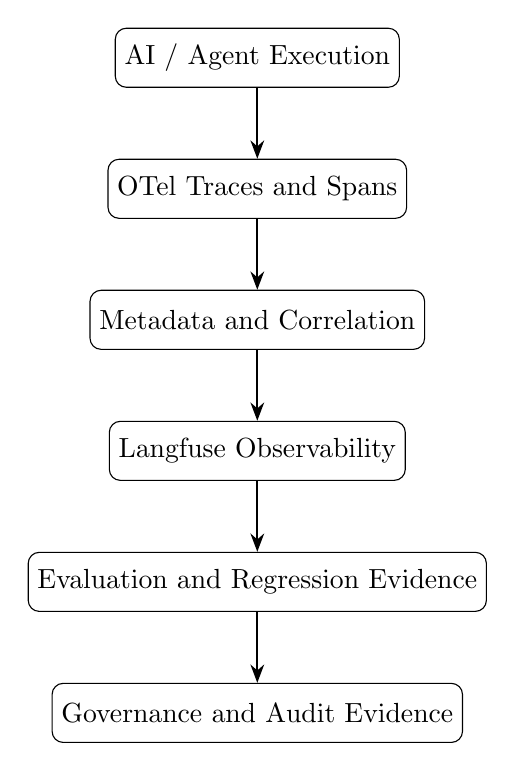
\begin{tikzpicture}[
node distance=0.9cm,
box/.style={
draw,
rounded corners,
minimum width=3.0cm,
minimum height=0.75cm,
align=center
},
arrow/.style={->,>=Stealth,thick}
]

\node[box] (execution) {AI / Agent Execution};
\node[box,below=of execution] (trace) {OTel Traces and Spans};
\node[box,below=of trace] (metadata) {Metadata and Correlation};
\node[box,below=of metadata] (observability) {Langfuse Observability};
\node[box,below=of observability] (evaluation) {Evaluation and Regression Evidence};
\node[box,below=of evaluation] (governance) {Governance and Audit Evidence};

\draw[arrow] (execution) -- (trace);
\draw[arrow] (trace) -- (metadata);
\draw[arrow] (metadata) -- (observability);
\draw[arrow] (observability) -- (evaluation);
\draw[arrow] (evaluation) -- (governance);

\end{tikzpicture}
}
\end{center}

The most important conclusion is:

\[
\boxed{
\text{If we cannot reconstruct how an AI system executed,}
}
\]

then:

\[
\boxed{
\text{debugging, evaluation, accountability, and auditing become much harder.}
}
\]

But the inverse is also important:

\[
\boxed{
\text{Being able to reconstruct execution does not, by itself, make the system governed.}
}
\]

A mature AI system therefore needs both:

\[
\boxed{
\text{Operational Visibility} + \text{Governance Controls}
}
\]

with structured telemetry serving as an important bridge between the two.

\end{document}